\documentclass[a4paper,10pt]{article}

\PassOptionsToPackage{fleqn}{amsmath}
\PassOptionsToPackage{normalem}{ulem}
\usepackage{Mathematics}

\usepackage[version=4]{mhchem}
\usepackage{longtable,booktabs}
\usepackage{xurl}
\usetikzlibrary{positioning}

\pdftitle{Chemistry -- HSLU, Semester 5}
\setcounter{tocdepth}{2}
\setlist[enumerate]{label=\textbf{\arabic*.},leftmargin=*}
\setlist[itemize]{leftmargin=*}
\setlength{\emergencystretch}{2em}
\renewcommand{\arraystretch}{1.2}
\newcolumntype{L}{>{\raggedright\arraybackslash}X}
\newcolumntype{P}[1]{>{\raggedright\arraybackslash}p{#1}}
\setchemfig{atom sep=2.2em,bond style={line width=0.6pt}}

\newcommand{\notebox}[1]{\begin{center}\fbox{%
  \begin{minipage}{\dimexpr\linewidth-2\fboxsep-2\fboxrule\relax}
  #1\end{minipage}}\end{center}}
\newcommand{\source}[1]{{\small\textit{Course source: #1.}\par}}
\newcommand{\chemunit}[1]{\,\mathrm{#1}}
\newcommand{\orbital}[1]{\fbox{\makebox[1.25em]{\ensuremath{#1}}}}
\newcommand{\chapterbreak}{\clearpage}

\title{\textbf{Chemistry -- 100\% AI SLOPPED!\\ HSLU, Semester 5}}
\author{Matteo Frongillo}
\date{}

\begin{document}
% Mathematics.sty puts a full-width author block in the title's tabular.
% Remove the tabular's outer padding locally so that it fits the text width.
\begingroup
\setlength{\tabcolsep}{0pt}
\maketitle
\endgroup
\tableofcontents
\chapterbreak

\section*{Scope and notation}
\addcontentsline{toc}{section}{Scope and notation}
These notes follow the theory material in \texttt{TA.BA\_CHEM\_MM.H2602}:
introduction to matter, atomic structure and radioactivity, atomic models,
the periodic table, electron configurations, chemical bonds, Lewis structures,
and chemical reactions (weeks 1--6). Exercise sheets, solution sheets and
exercise prompts inside the lectures are excluded. Small molecular illustrations
are included to explain the theory.

The supplied formula sheet and MEP reference notes also contain acid--base
and electrochemical material. This is collected in
Appendices~\ref{app:acidbase} and~\ref{app:redox}; it is reference material,
not a reconstruction of lecture weeks that are absent from the folder.
A source map is provided in Appendix~\ref{app:sources}.

\begin{tabularx}{\linewidth}{@{}lLlL@{}}
\toprule
Symbol & Meaning & Symbol & Meaning \\
\midrule
$m$ & Mass & $n$ & Amount of substance \\
$N$ & Number of specified particles & $N_{\mathrm A}$ & Avogadro constant \\
$M$ & Molar mass & $c$ & Amount concentration (molarity) \\
$V$ & Volume & $\rho$ & Density \\
$Z$ & Atomic number & $A$ & Mass number \\
$T$ & Absolute temperature in kelvin & $p$ & Absolute pressure \\
\bottomrule
\end{tabularx}

The lecture material sometimes uses $M$ for molarity. Here $M$ always denotes
molar mass and $c$ denotes molarity, to keep the two quantities distinct.
Chemical formulas and equations use \texttt{mhchem}; molecular drawings use
\texttt{chemfig}. A line represents a shared electron pair and a pair of dots
represents a lone pair.

\section{Substances and mixtures}
\label{sec:matter}
\source{SW1, Introduction to Substances}

\subsection{Classification of matter}
\textbf{Matter} has mass and occupies space. Its classification depends on
composition and on whether its properties are uniform throughout the sample.
\begin{itemize}
  \item A \textbf{pure substance} has a fixed chemical composition and characteristic
  properties at specified temperature and pressure.
  \item An \textbf{element} contains atoms with the same atomic number and cannot
  be decomposed into simpler substances by chemical methods.
  \item A \textbf{compound} contains two or more elements in a fixed ratio.
  Chemical reactions can decompose it into other substances.
  \item A \textbf{mixture} contains several substances in variable proportions.
  Its components can be separated using differences in physical properties.
\end{itemize}

\begin{center}
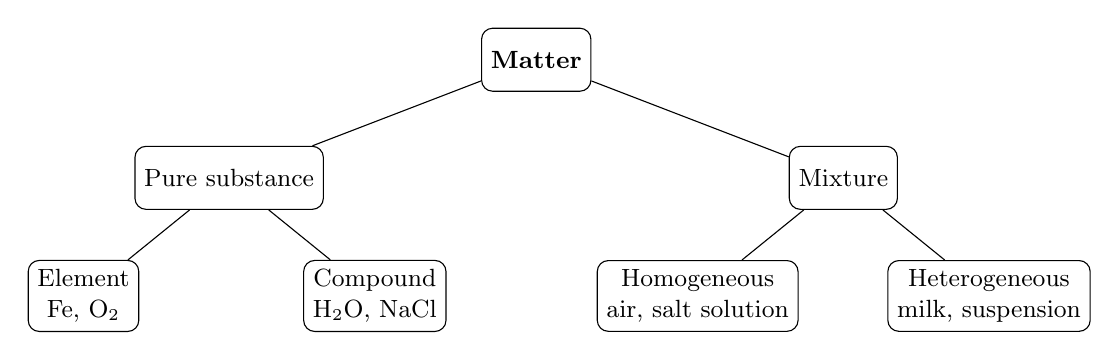
\begin{tikzpicture}[every node/.style={draw,rounded corners,align=center,
  font=\small,minimum height=8mm},level distance=15mm,
  level 1/.style={sibling distance=78mm},level 2/.style={sibling distance=37mm}]
\node {\textbf{Matter}}
 child {node {Pure substance}
   child {node {Element\\\ce{Fe}, \ce{O2}}}
   child {node {Compound\\\ce{H2O}, \ce{NaCl}}}}
 child {node {Mixture}
   child {node {Homogeneous\\air, salt solution}}
   child {node {Heterogeneous\\milk, suspension}}};
\end{tikzpicture}
\end{center}

A \textbf{homogeneous mixture} is uniform on the scale considered and forms
one phase. A \textbf{heterogeneous mixture} contains distinguishable phases;
these need not be visible to the naked eye. Milk, for example, is an emulsion.
A \textbf{phase} is a region with uniform physical and chemical properties.

\begin{tabularx}{\linewidth}{@{}lLL@{}}
\toprule
Mixture & Dispersed substance and medium & Example \\
\midrule
Solution & Molecular or ionic mixing in one phase & Salt water; air \\
Suspension & Solid particles in a liquid & Muddy water \\
Emulsion & Liquid droplets in another liquid & Milk; oil droplets in water \\
Aerosol & Liquid droplets or solid particles in a gas & Fog; smoke \\
Solid mixture & Several solid phases & Granite \\
\bottomrule
\end{tabularx}

\subsection{Physical, chemical and nuclear changes}
\begin{enumerate}
  \item A \textbf{physical change} alters the state, shape, size or distribution
  of substances without changing their chemical identity. Melting ice and
  separating a mixture are physical processes.
  \item A \textbf{chemical reaction} forms different substances through a
  rearrangement of atoms and electrons. Chemical bonds are broken and formed;
  atomic nuclei retain their identities.
  \item A \textbf{nuclear reaction} changes a nucleus. It may change the element
  and involves much larger characteristic energies per event than chemical reactions.
\end{enumerate}
\notebox{\textbf{Distinguishing criterion:} ask whether new substances form.
Reversibility alone does not distinguish physical from chemical changes.
Breaking glass is physical, while a chemical reaction can be reversible.}

Physical properties include density, melting temperature and conductivity.
Chemical properties describe reactivity, such as the tendency to burn or oxidize.
An \textbf{extensive} quantity depends on sample size (mass, volume);
an \textbf{intensive} quantity does not (temperature, density of a uniform phase).

\subsection{Separation methods}

\begin{tabularx}{\linewidth}{@{}P{27mm}LL@{}}
\toprule
Method & Property used & Principle or application \\
\midrule
Sedimentation & Density and particle settling & Suspended solids settle under gravity;
used in wastewater treatment. \\
Decantation & Separated phases & Pour off a liquid above a settled solid, or separate
immiscible liquid layers using a separating funnel. \\
Filtration & Particle size & A porous medium retains the residue; the fluid passing
through is the filtrate. Dissolved ions pass through ordinary filters. \\
Distillation & Relative volatility & Vaporize and condense a mixture to obtain a
distillate enriched in more volatile components. \\
Extraction & Different solubilities & Transfer a substance into a suitable solvent;
for example, extracting soluble compounds from tea. \\
Adsorption & Affinity for a surface & Substances bind to a solid surface, as in
activated-carbon treatment. \\
Absorption & Uptake into a bulk phase & A gas dissolves in a liquid absorbent,
as in gas scrubbing. \\
\bottomrule
\end{tabularx}

\textbf{Adsorption} occurs at a surface; \textbf{absorption} occurs throughout
the absorbing phase. In practice, several separation steps are often combined.

\subsection{States of matter and phase transitions}

\begin{tabularx}{\linewidth}{@{}lLLL@{}}
\toprule
State & Shape & Volume & Particle picture \\
\midrule
Solid & Approximately fixed & Approximately fixed & Particles vibrate near fixed positions. \\
Liquid & Container shape & Approximately fixed & Closely packed particles can move past one another. \\
Gas & Fills container & Container volume & Widely separated particles move freely. \\
Plasma & No fixed shape & No fixed volume & Contains mobile ions and electrons; conducts electricity. \\
\bottomrule
\end{tabularx}

\begin{center}
\begin{tikzpicture}[>=Stealth,every node/.style={font=\small}]
\node[draw,rounded corners,minimum width=22mm,minimum height=10mm] (s) at (0,0) {Solid};
\node[draw,rounded corners,minimum width=22mm,minimum height=10mm] (l) at (5,0) {Liquid};
\node[draw,rounded corners,minimum width=22mm,minimum height=10mm] (g) at (10,0) {Gas};
\draw[->] ([yshift=2mm]s.east) -- node[above]{Melting} ([yshift=2mm]l.west);
\draw[->] ([yshift=-2mm]l.west) -- node[below]{Freezing} ([yshift=-2mm]s.east);
\draw[->] ([yshift=2mm]l.east) -- node[above]{Vaporization} ([yshift=2mm]g.west);
\draw[->] ([yshift=-2mm]g.west) -- node[below]{Condensation} ([yshift=-2mm]l.east);
\draw[->] (s.north) to[bend left=24] node[above]{Sublimation} (g.north);
\draw[->] (g.south) to[bend left=24] node[below]{Deposition} (s.south);
\end{tikzpicture}
\end{center}
Melting, vaporization and sublimation absorb heat; the reverse processes release
heat. During a phase transition of a pure substance at constant pressure,
heat changes the phase fraction while the temperature remains constant.

\subsection{Reading a phase diagram}
A phase diagram shows the stable phase as a function of pressure and temperature.
Inside a region, one phase is stable; on a boundary, two phases coexist.
\begin{itemize}
  \item At the \textbf{triple point}, solid, liquid and gas coexist.
  \item At the \textbf{critical point}, the liquid--gas coexistence curve ends.
  Above the critical temperature, pressure alone cannot produce a distinct liquid phase.
  \item Heating at constant pressure follows a horizontal path on a $p$--$T$ diagram.
  Compression at constant temperature follows a vertical path.
\end{itemize}
For water near atmospheric pressure, increasing pressure lowers the melting
temperature because liquid water is denser than ordinary ice. This gives the
solid--liquid boundary a negative slope in that region.

\begin{center}
\begin{tikzpicture}[>=Stealth,x=1cm,y=1cm,font=\small]
\draw[->] (0,0) -- (8.2,0) node[right] {$T$};
\draw[->] (0,0) -- (0,4.6) node[above] {$p$};
\draw[thick] (0.4,0.2) .. controls (1.3,0.35) and (2,0.8) .. (2.6,1.3);
\draw[thick] (2.6,1.3) -- (1.8,4.2);
\draw[thick] (2.6,1.3) .. controls (4.8,1.6) and (6,2.6) .. (7,3.9);
\fill (2.6,1.3) circle (2pt) node[below right]{Triple point};
\fill (7,3.9) circle (2pt) node[above]{Critical point};
\node at (1,2.5) {Solid}; \node at (3.9,3.2) {Liquid};
\node at (5.6,0.6) {Gas};
\draw[->,dashed] (0.7,2.2) -- (7.2,2.2);
\end{tikzpicture}

{\small Schematic phase diagram for water near the familiar phase boundaries;
not to scale. The dashed path illustrates heating at fixed pressure.}
\end{center}

\subsection{Density and the anomaly of water}
\figbox{$\displaystyle \rho=\frac{m}{V},\qquad m=\rho V$}
Common units are $\mathrm{kg\,m^{-3}}$ and $\mathrm{g\,cm^{-3}}$:
$1\chemunit{g\,cm^{-3}}=1000\chemunit{kg\,m^{-3}}$.
Density depends on temperature and pressure, especially for gases.
At ordinary pressure, liquid water has its maximum density near $4\,^{\circ}\mathrm C$.
Ordinary ice is less dense than liquid water and therefore floats. Its open
hydrogen-bonded structure explains the expansion on freezing.

\chapterbreak
\section{Amount of substance and solutions}
\label{sec:solutions}
\source{SW1 and the supplied formula sheet, items 1--4}

\subsection{Atomic, molecular and molar mass}
The \textbf{atomic mass constant} $m_{\mathrm u}$ is one twelfth of the mass of a
free carbon-12 atom in its ground state and at rest. The unified atomic mass unit
is $1\chemunit{u}=m_{\mathrm u}\approx1.66054\times10^{-27}\chemunit{kg}$.

The \textbf{relative atomic mass} $A_{\mathrm r}$ is dimensionless:
\[
 A_{\mathrm r}=\frac{\overline m_{\mathrm{atom}}}{m_{\mathrm u}},
 \qquad \overline m_{\mathrm{atom}}=\sum_i x_i m_i,
 \qquad \sum_i x_i=1.
\]
Here $x_i$ is the abundance fraction of isotope $i$, and $m_i$ its atomic mass.
The periodic table usually gives an abundance-weighted atomic weight, not the
integer mass number of a particular isotope.

For a molecule, add the atomic masses with their formula subscripts as multipliers.
For an ionic solid, the corresponding quantity is a \textbf{formula mass}, since
the solid is a lattice rather than a collection of isolated molecules.
\figbox{$\displaystyle
 M(\ce{A_{p}B_{q}C_{r}})=pM(\ce{A})+qM(\ce{B})+rM(\ce{C})$}
For example, $M(\ce{H2O})=2M(\ce{H})+M(\ce{O})\approx18.015\chemunit{g\,mol^{-1}}$.
At the precision used in this course, the numerical mass of a particle in
$\mathrm u$ equals the numerical molar mass in $\mathrm{g\,mol^{-1}}$.

\subsection{The mole and Avogadro constant}
The \textbf{mole} measures the amount of specified entities: atoms, molecules,
ions, electrons or formula units. One mole contains exactly
$6.02214076\times10^{23}$ such entities (the SI definition; see
Appendix~\ref{app:sources}).
\figbox{$\displaystyle
 N_{\mathrm A}=6.02214076\times10^{23}\chemunit{mol^{-1}},\qquad
 n=\frac{N}{N_{\mathrm A}}=\frac{m}{M},\qquad N=nN_{\mathrm A}$}
Always specify what is being counted: one mole of \ce{O2} molecules contains two
moles of oxygen atoms. For \ce{NaCl}, count formula units or the individual ions,
according to the question.

\subsection{Solutions and solubility}
A \textbf{solution} is a homogeneous mixture. The \textbf{solvent} is the dissolving
medium, commonly the component present in the largest amount. A \textbf{solute}
is a dissolved component. Solvent molecules surround dissolved particles;
this is \textbf{solvation}, or \textbf{hydration} when the solvent is water.

\textbf{Solubility} is the equilibrium amount of a solute that can dissolve under
specified conditions. State the temperature, pressure where relevant, and the
concentration basis (for example, grams per litre of solution or per 100 g of solvent).
\begin{itemize}
  \item \textbf{Unsaturated:} more solute can dissolve.
  \item \textbf{Saturated:} the dissolved concentration equals the solubility;
  with excess solid present, dissolution and crystallization balance.
  \item \textbf{Supersaturated:} the concentration exceeds the equilibrium value.
  Such a solution is metastable and can crystallize after a disturbance or seeding.
\end{itemize}

\subsubsection{Energy of dissolution}
Dissolution requires separating solute particles and rearranging solvent
interactions, while forming solute--solvent interactions releases energy.
\[
 \Delta H_{\mathrm{sol}}=
 \Delta H_{\mathrm{separate\ solute}}+
 \Delta H_{\mathrm{rearrange\ solvent}}+
 \Delta H_{\mathrm{solvation}}.
\]
The net process can be exothermic or endothermic. Solubility is governed by the
free-energy balance, not only by the speed of dissolution. Heating often increases
the solubility of solids, but this is not a universal rule.

\subsubsection{Gas solubility}
For a dilute solution of a gas that does not react significantly with the solvent,
Henry's law can be written
\figbox{$\displaystyle c_{\mathrm{gas}}=k_{\mathrm H}p_{\mathrm{gas}}$
\quad (fixed temperature)}
Here $p_{\mathrm{gas}}$ is the gas's \textbf{partial pressure} above the solution;
the units and value of $k_{\mathrm H}$ depend on the chosen convention.
Gas solubility generally increases with partial pressure and decreases with
temperature. A pressure decrease can therefore release dissolved gas as bubbles.

\subsection{Concentration units}
\label{sec:concentration}

\begin{tabularx}{\linewidth}{@{}P{34mm}P{64mm}L@{}}
\toprule
Quantity & Definition & Typical unit or convention \\
\midrule
Molarity & $c=n_{\mathrm{solute}}/V_{\mathrm{solution}}$ & $\mathrm{mol\,L^{-1}}$ \\
Mass concentration & $\beta=m_{\mathrm{solute}}/V_{\mathrm{solution}}$ & $\mathrm{g\,L^{-1}}$ \\
Mass fraction & $w=m_{\mathrm{solute}}/m_{\mathrm{solution}}$ & Dimensionless; mass percentage $=100w\,\%$ \\
Volume percentage & $100V_{\mathrm{solute}}/V_{\mathrm{solution}}$ & $\%$ by volume; specify temperature \\
Mass/volume percentage & Grams of solute per $100\chemunit{mL}$ of solution & $\%\,(m/V)$; not dimensionless \\
Parts per million & $10^6w$ on a mass basis & $1\chemunit{ppm}=1\chemunit{mg\,kg^{-1}}$ \\
Parts per billion & $10^9w$ on a mass basis & $1\chemunit{ppb}=1\,\si{\micro\gram\per\kilogram}$ \\
\bottomrule
\end{tabularx}

For dilute aqueous solutions with $\rho\approx1\chemunit{kg\,L^{-1}}$,
$1\chemunit{mg\,L^{-1}}\approx1\chemunit{ppm}$ on a mass basis. This equivalence is
an approximation and does not apply to arbitrary liquids or gas mixtures.
\figbox{$\displaystyle c=\frac{m}{MV},\qquad \beta=cM,\qquad
 c=\frac{w\rho}{M}$}
Use consistent units: if $\rho$ is in $\mathrm{g\,L^{-1}}$ and $M$ in
$\mathrm{g\,mol^{-1}}$, the last expression gives $c$ in $\mathrm{mol\,L^{-1}}$.
The denominator in molarity is the volume of the \textbf{final solution}, not
the volume of solvent initially added.

\subsection{Preparing and diluting solutions}
To prepare a solution from a solid, calculate $m=cMV$, dissolve the weighed
solute in part of the solvent, then make up to the required final volume.
For a dilution, the solute amount is conserved if no reaction or loss occurs:
\figbox{$\displaystyle n_1=n_2\quad\Longrightarrow\quad
 c_1V_1=c_2V_2,\qquad V_1=\frac{c_2V_2}{c_1}$}
$V_1$ is the stock-solution aliquot and $V_2$ the final diluted volume.
Adding solvent lowers concentration, but does not change the amount of solute.
Volumes are not always exactly additive when different liquids are mixed.

\notebox{\textbf{Keep separate:} concentration describes how much solute is
present; solubility describes the equilibrium limit. A concentrated solution
need not be saturated, and a saturated solution can have a very low concentration.}

\chapterbreak
\section{Atomic structure and radioactivity}
\label{sec:atoms}
\source{SW2, Structure of atoms}

\subsection{The nucleus and electron cloud}
An atom contains a small, massive nucleus and an electron cloud that determines
most of its size. Typical atomic dimensions are of order $10^{-10}\chemunit m$,
whereas nuclear dimensions are of order $10^{-15}$--$10^{-14}\chemunit m$.
\begin{center}
\begin{tabular}{@{}llll@{}}
\toprule
Particle & Charge & Approximate mass & Location \\
\midrule
Proton & $+e$ & $1.0073\chemunit u$ & Nucleus \\
Neutron & $0$ & $1.0087\chemunit u$ & Nucleus \\
Electron & $-e$ & $0.0005486\chemunit u$ & Electron cloud \\
\bottomrule
\end{tabular}
\end{center}
Almost all atomic mass is in the nucleus. The number of protons identifies the
element; electron arrangement is central to its chemical behaviour.

\subsection{Nuclide notation and ions}
\figbox{$\displaystyle {}^{A}_{Z}\mathrm X^{q},\qquad
 A=Z+N_{\mathrm n},\qquad N_{\mathrm n}=A-Z,\qquad N_{\mathrm e}=Z-q$}
Here $q$ is the signed charge number ($+2$ for a doubly positive ion),
$N_{\mathrm n}$ the neutron count and $N_{\mathrm e}$ the electron count.
For a neutral atom, $N_{\mathrm e}=Z$.
\begin{itemize}
  \item A \textbf{cation} forms by electron loss and has positive charge.
  \item An \textbf{anion} forms by electron gain and has negative charge.
  \item Forming an ion does not change the number of protons or the element.
\end{itemize}
\[
 \ce{Na -> Na+ + e-},\qquad \ce{Cl + e- -> Cl-}.
\]

\subsection{Isotopes and isobars}
\textbf{Isotopes} have the same $Z$ but different neutron counts and mass numbers.
For example, $^{12}_{6}\mathrm C$, $^{13}_{6}\mathrm C$ and $^{14}_{6}\mathrm C$
contain 6, 7 and 8 neutrons. \textbf{Isobars} have the same mass number $A$
but different atomic numbers.

Hydrogen isotopes have special names: \textbf{protium} $^{1}_{1}\mathrm H$,
\textbf{deuterium} $^{2}_{1}\mathrm H$ and \textbf{tritium} $^{3}_{1}\mathrm H$.
Isotopes have similar electronic structures and broadly similar chemistry,
but their different masses can affect reaction rates and physical properties.
Some isotopes are radioactive, while others are stable.

\subsection{Radioactive decay}
An unstable nucleus can transform spontaneously and emit ionizing radiation.
Nuclear stability depends on both size and neutron-to-proton ratio; light stable
nuclei often have comparable neutron and proton counts, while heavier stable
nuclei require a neutron excess.

\subsubsection{Alpha decay}
The emitted alpha particle is a helium nucleus containing two protons and two neutrons:
\figbox{$\displaystyle {}^{A}_{Z}\mathrm X\longrightarrow
 {}^{A-4}_{Z-2}\mathrm Y+{}^{4}_{2}\mathrm{He}$}
$A$ decreases by four and $Z$ by two. Alpha radiation has high ionization density
and a short range in matter.

\subsubsection{Beta decay}
In \textbf{beta-minus decay}, a neutron becomes a proton, emitting an electron
and an electron antineutrino:
\[
 \mathrm n\longrightarrow\mathrm p+\mathrm e^-+\overline\nu_{\mathrm e},
 \qquad {}^{A}_{Z}\mathrm X\longrightarrow{}^{A}_{Z+1}\mathrm Y
 +{}^{0}_{-1}\mathrm e+\overline\nu_{\mathrm e}.
\]
$A$ is unchanged and $Z$ increases by one. The emitted electron is produced
in the decay; it is not an orbital electron leaving the atom.
In \textbf{beta-plus decay}, a proton becomes a neutron with emission of a
positron and a neutrino, so $Z$ decreases by one while $A$ stays unchanged.

\subsubsection{Gamma emission}
An excited nucleus loses energy by emitting a photon:
\figbox{$\displaystyle {}^{A}_{Z}\mathrm X^{*}\longrightarrow
 {}^{A}_{Z}\mathrm X+\gamma$}
Neither $A$ nor $Z$ changes. Gamma emission often follows an alpha or beta decay.

\begin{tabularx}{\linewidth}{@{}lLL@{}}
\toprule
Radiation & Nature & Qualitative penetration \\
\midrule
$\alpha$ & Helium nuclei & Short range; stopped by paper or the outer skin layer. \\
$\beta$ & Electrons or positrons & More penetrating than alpha; range depends strongly on energy. \\
$\gamma$ & High-energy photons & Highly penetrating; attenuated by substantial thicknesses of dense material. \\
\bottomrule
\end{tabularx}

These are qualitative comparisons, not shielding specifications. The effect of
radiation depends on its energy, exposure and whether radioactive material is
outside or inside an object or organism. Radon is an example of a radioactive
gas that can migrate from the ground into buildings.

\subsection{Half-life and activity}
For a single radionuclide with no replenishment, the decay rate is proportional
to the number of undecayed nuclei:
\figbox{$\displaystyle
 N(t)=N_0e^{-\lambda t}=N_0\left(\frac12\right)^{t/t_{1/2}},\qquad
 t_{1/2}=\frac{\ln2}{\lambda}$}
The \textbf{activity} $\mathcal A$ is the number of decays per unit time:
\[
 \mathcal A(t)=-\frac{\mathrm dN}{\mathrm dt}=\lambda N(t),\qquad
 1\chemunit{Bq}=1\chemunit{s^{-1}}.
\]
After one, two and three half-lives, $1/2$, $1/4$ and $1/8$ of the initial nuclei
remain. For the same number of radioactive nuclei, a shorter half-life means
a higher activity. For the same isotope, activity and remaining radioactive
mass decrease by the same factor.

\subsection{Radiocarbon dating}
Living organisms exchange carbon with their environment. After death, this
exchange ceases and the carbon-14 content decreases through beta-minus decay.
Using its approximate half-life of $5730\chemunit{years}$,
\figbox{$\displaystyle
 t=\frac{t_{1/2}}{\ln2}\ln\!\left(\frac{N_0}{N(t)}\right)
 =\frac{t_{1/2}}{\ln2}\ln\!\left(\frac{\mathcal A_0}{\mathcal A(t)}\right)$}
The simple relation assumes a known initial carbon-14 ratio and a closed sample.
Practical dating also requires calibration and correction for contamination.

\subsection{Fission, fusion and energy}
\textbf{Fission} splits a heavy nucleus into lighter nuclei, commonly releasing
neutrons that can trigger further fissions. A controlled chain reaction produces
heat in a nuclear reactor. \textbf{Fusion} combines light nuclei and powers stars.
Energy release is associated with an increase in nuclear binding energy:
\figbox{$\displaystyle E_{\mathrm{released}}=
 (m_{\mathrm{initial}}-m_{\mathrm{final}})c_0^2$}
Here $c_0$ is the speed of light, distinct from concentration $c$.
Balance mass numbers and atomic numbers in nuclear equations. Chemical reactions
rearrange electrons; nuclear reactions alter the nuclei themselves.
Applications discussed in the course include energy production, radiographic
inspection, tracers and radiation-assisted pollutant treatment.

\chapterbreak
\section{Atomic models and electron configuration}
\label{sec:orbitals}
\source{SW3, Atomic Models (self-study) and Electronic Configuration}

\subsection{Development of the atomic model}

\begin{tabularx}{\linewidth}{@{}P{24mm}LL@{}}
\toprule
Model & Main idea or observation & Limitation or development \\
\midrule
Dalton & Matter consists of atoms; chemical reactions rearrange them in simple
ratios. & Atoms are not indivisible, and isotopes of an element have different masses. \\
Thomson & Cathode rays reveal electrons; negative particles are embedded in a
positive background. & Does not account for the concentrated atomic nucleus. \\
Rutherford & Most alpha particles pass through gold foil, while a few deflect
strongly: a tiny positive nucleus contains most mass. & Classical orbiting electrons
do not explain stable atoms and discrete spectra. \\
Bohr & Electrons occupy discrete energy levels; transitions absorb or emit light.
& Useful for hydrogen-like atoms, but insufficient for general many-electron atoms. \\
Quantum model & Electrons are described by wavefunctions and orbitals rather
than fixed trajectories. & Probability distributions replace classical paths. \\
\bottomrule
\end{tabularx}

For an electronic transition, the photon energy is
\[
 E_{\mathrm{photon}}=h\nu=\frac{hc_0}{\lambda_{\mathrm{light}}}
 =\lvert E_{\mathrm{final}}-E_{\mathrm{initial}}\rvert.
\]
An upward transition absorbs energy; a downward transition emits it.
Characteristic energy differences explain line spectra and flame colours.

\subsection{Orbitals and quantum numbers}
An \textbf{orbital} is a one-electron wavefunction. Its squared magnitude
$|\psi|^2$ gives a probability density; an orbital drawing usually encloses a
chosen fraction of that probability. An orbital is not an electron's path.
The uncertainty principle constrains position and momentum simultaneously:
\[
 \Delta x\,\Delta p_x\geq\frac{\hbar}{2}.
\]

\begin{tabularx}{\linewidth}{@{}P{35mm}P{47mm}L@{}}
\toprule
Quantum number & Allowed values & Meaning \\
\midrule
Principal, $n$ & $1,2,3,\ldots$ & Shell; characteristic size and energy scale. \\
Angular momentum, $\ell$ & $0,1,\ldots,n-1$ & Subshell and orbital shape. \\
Magnetic, $m_\ell$ & $-\ell,\ldots,0,\ldots,+\ell$ & Orbital orientation; $2\ell+1$ values. \\
Spin projection, $m_s$ & $+\tfrac12$ or $-\tfrac12$ & Two possible spin projections for an electron. \\
\bottomrule
\end{tabularx}

Spin is an intrinsic quantum property, not a literal classical rotation of the
electron. The electron has spin quantum number $s=1/2$; the two alternatives
above are the projections $m_s$.

\begin{center}
\begin{tabular}{@{}ccclc@{}}
\toprule
Subshell & $\ell$ & Orbitals & Shape (schematic description) & Maximum electrons \\
\midrule
s & 0 & 1 & Spherical & 2 \\
p & 1 & 3 & Two lobes & 6 \\
d & 2 & 5 & Mostly four lobes & 10 \\
f & 3 & 7 & More complex angular shapes & 14 \\
\bottomrule
\end{tabular}
\end{center}
\figbox{$\displaystyle
 \text{Orbitals in shell }n=n^2,\qquad
 \text{maximum electrons in shell }n=2n^2$}
The first four shells have capacities 2, 8, 18 and 32. These are capacities,
not the order in which the ground-state atom fills the subshells.

\subsection{Filling rules}
\begin{enumerate}
  \item \textbf{Aufbau principle:} occupy lower-energy orbitals first.
  The usual order is summarized below; some atoms have exceptions.
  \item \textbf{Pauli exclusion principle:} no two electrons in an atom have
  the same four quantum numbers. Each orbital holds at most two electrons,
  with opposite spins.
  \item \textbf{Hund's rule:} occupy degenerate orbitals singly with parallel
  spins before pairing electrons.
\end{enumerate}
\figbox{$\begin{gathered}
 1\mathrm s\to2\mathrm s\to2\mathrm p\to3\mathrm s\to3\mathrm p\to4\mathrm s
 \to3\mathrm d\to4\mathrm p\to5\mathrm s\\
 \to4\mathrm d\to5\mathrm p\to6\mathrm s\to4\mathrm f\to5\mathrm d\to6\mathrm p
 \to7\mathrm s\to5\mathrm f\to6\mathrm d\to7\mathrm p
\end{gathered}$}
The $(n+\ell)$ rule is a useful guide: fill smaller $n+\ell$ first, with smaller
$n$ breaking ties. Actual subshell energies also depend on occupancy.

A $\mathrm p^3$ subshell illustrates Hund's rule:
\begin{center}
\orbital{\uparrow}\ \orbital{\uparrow}\ \orbital{\uparrow}
\qquad rather than \qquad
\orbital{\uparrow\downarrow}\ \orbital{\uparrow}\ \orbital{}
\end{center}
For $\mathrm p^4$, one pair is necessary:
\begin{center}
\orbital{\uparrow\downarrow}\ \orbital{\uparrow}\ \orbital{\uparrow}.
\end{center}

\subsection{Writing a configuration}
Determine the number of electrons, fill subshells in order, and check that the
superscripts sum to the electron count. A noble-gas symbol in brackets replaces
the filled core. For example,
\[
 \ce{Si}:\quad 1\mathrm s^2\,2\mathrm s^2\,2\mathrm p^6\,3\mathrm s^2\,3\mathrm p^2
 =[\ce{Ne}]\,3\mathrm s^2\,3\mathrm p^2.
\]
For main-group atoms, the outermost s and p electrons are the
\textbf{valence electrons}. Core electrons occupy the inner filled shells.
Transition-metal bonding can also involve the $(n-1)\mathrm d$ electrons.

When forming a cation, remove electrons from the outermost occupied shell first.
For transition-metal cations, the $n\mathrm s$ electrons are normally removed
before $(n-1)\mathrm d$ electrons, even though $n\mathrm s$ was filled first.
Anions gain electrons subject to the same occupancy rules.
Configurations with nearby s and d energies can depart from the simple filling
sequence; use the supplied periodic-table data when such exceptions are relevant.

\chapterbreak
\section{The periodic table}
\label{sec:periodic}
\source{SW3, Periodic Table; MEP notes, oxidation-number reference}

\subsection{Periods, groups and blocks}
Elements are ordered by increasing \textbf{atomic number} $Z$.
\textbf{Periods} are the seven horizontal rows; \textbf{groups} are the 18 vertical
columns. Main-group elements in the same group have similar valence-shell
configurations, which helps explain their related chemical properties.

The s, p, d and f blocks identify the subshell being populated across a series.
For main-group atoms, the period corresponds to the highest occupied principal
shell in the usual ground-state configuration. The group number gives the
valence-electron count for groups 1 and 2, and group number minus ten for groups
13--18. Helium is the exception: its full shell is $1\mathrm s^2$.

\begin{tabularx}{\linewidth}{@{}P{29mm}P{26mm}L@{}}
\toprule
Family & Outer configuration & Characteristic behaviour \\
\midrule
Group 1: alkali metals & $n\mathrm s^1$ & Easily lose one electron; usually form $+1$
ions. Reactivity generally increases down the group. Hydrogen is not an alkali metal. \\
Group 2: alkaline-earth metals & $n\mathrm s^2$ & Usually form $+2$ ions; reducing
metals, generally less reactive than neighbouring alkali metals. \\
Group 17: halogens & $n\mathrm s^2n\mathrm p^5$ & Commonly form $-1$ ions;
\ce{F2}, \ce{Cl2}, \ce{Br2}, \ce{I2} are diatomic. Oxidizing ability generally
decreases down the group. \\
Group 18: noble gases & $n\mathrm s^2n\mathrm p^6$ & Filled valence shell (He:
$1\mathrm s^2$); very low reactivity, but not universally incapable of bonding. \\
\bottomrule
\end{tabularx}

\subsection{Metals, nonmetals and metalloids}
\textbf{Metals} occupy most of the left and centre of the table. They generally
conduct heat and electricity, are malleable and ductile, and tend to lose
electrons. \textbf{Nonmetals} occupy mainly the upper right and have diverse
properties; many are poor electrical conductors. \textbf{Metalloids}, near the
boundary, have intermediate properties and include useful semiconductors.

\subsection{Periodic trends}
Across a period, the nuclear charge increases while added electrons mainly
enter the same shell. The increasing effective nuclear attraction generally
pulls valence electrons closer. Down a group, extra shells and shielding
increase the distance of valence electrons from the nucleus.

\begin{tabularx}{\linewidth}{@{}P{41mm}LL@{}}
\toprule
Property & Left to right across a period & Top to bottom down a group \\
\midrule
Atomic radius & Generally decreases & Generally increases \\
First ionization energy & Generally increases & Generally decreases \\
Electronegativity & Generally increases & Generally decreases \\
Metallic character & Generally decreases & Generally increases \\
\bottomrule
\end{tabularx}

These are trends, not exact rules for every adjacent pair. Subshell structure,
electron pairing and the definition of atomic radius can produce exceptions.

\textbf{Ionization energy} is the energy required to remove an electron from a
gaseous atom or ion. The first ionization is
\[
 \ce{X(g) -> X+(g) + e-}.
\]
Successive ionizations require increasing energy; a large jump often marks
the start of removing a core electron.

\textbf{Electronegativity} describes an atom's tendency to attract shared
electrons in a bond. It is not the same as ionization energy. Fluorine has the
highest electronegativity on the commonly used Pauling scale.

Cations are generally smaller than their neutral parent atoms; anions are
larger. Among \textbf{isoelectronic} species (same electron count), increasing
nuclear charge generally decreases radius.

\subsection{Oxidation numbers}
\label{sec:oxidation}
An \textbf{oxidation number} assigns bonding electrons to the more
electronegative atom, as if the bond were completely ionic. It is a bookkeeping
quantity and is not necessarily an actual atomic charge.
\begin{enumerate}
  \item An element in its elemental form has oxidation number zero.
  \item A monatomic ion has an oxidation number equal to its signed charge number.
  \item Fluorine is $-1$ in its compounds. Group 1 and group 2 metals are usually
  $+1$ and $+2$, respectively, in their compounds.
  \item Hydrogen is usually $+1$, but is $-1$ in metal hydrides.
  \item Oxygen is usually $-2$; in peroxides it is $-1$. Oxygen bonded to fluorine
  can have a positive oxidation number.
  \item The sum, including the number of each atom, equals the overall charge:
\end{enumerate}
\figbox{$\displaystyle \sum_i n_i\,\mathrm{OS}_i=q_{\mathrm{species}}$}
For example, sulfur in \ce{SO4^2-} satisfies
$\mathrm{OS}_{\mathrm S}+4(-2)=-2$, hence $\mathrm{OS}_{\mathrm S}=+6$.
Do not apply a compound rule to a free element: oxygen in \ce{O2} has oxidation
number zero, not $-2$.

\begin{center}
\begin{tabular}{@{}ll@{}}
\toprule
Element & Selected common oxidation numbers in compounds \\
\midrule
C & $-4,+2,+4$ \\
N & $-3,+2,+3,+4,+5$ \\
P & $-3,+3,+5$ \\
S & $-2,+2,+4,+6$ \\
Cl, Br, I & $-1,+1,+3,+5,+7$ \\
Zn & $+2$ \\
Pb & $+2,+4$ \\
\bottomrule
\end{tabular}
\end{center}
These lists are useful common values, not exhaustive sets of possible states.
Redox reactions change oxidation numbers (Appendix~\ref{app:redox}).

\subsection{Abundance of elements}
Hydrogen and helium dominate ordinary matter in the cosmos. Oxygen and silicon
are major constituents of Earth's crust. Oxygen, carbon, hydrogen and nitrogen
account for about $96\%$ of human body mass. Always distinguish mass fractions
from fractions of atoms when comparing elemental abundances.

\chapterbreak
\section{Chemical bonds and hybridization}
\label{sec:bonds}
\source{SW4, Chemical Bonds and Hybridization; SW5 recap}

\subsection{Why atoms bond}
A stable bond corresponds to a lower energy than the separated atoms under
the conditions considered. Attraction between nuclei and electrons competes
with electron--electron and nucleus--nucleus repulsion. The minimum of the
potential-energy curve defines an equilibrium bond length.

\begin{center}
\begin{tikzpicture}[>=Stealth,font=\small]
\draw[->] (0,-2.3) -- (7.6,-2.3) node[right]{Nuclear separation $r$};
\draw[->] (0,-2.3) -- (0,2.3) node[above]{Potential energy};
\draw[dashed] (0,0) -- (7.2,0) node[right]{$0$};
\draw[thick] (0.8,2) .. controls (1.1,0) and (1.3,-1.8) .. (2,-1.8)
 .. controls (3,-1.8) and (4,-0.1) .. (7,-0.04);
\draw[dashed] (2,-1.8) -- (2,-2.3) node[below]{$r_{\mathrm e}$};
\draw[<->] (2,0) -- (2,-1.8) node[midway,right]{Bond-well depth};
\node at (5.1,1.1){Separated atoms};
\end{tikzpicture}
\end{center}
Bond formation releases energy; separating a stable bond requires energy.
The energy change of a whole reaction depends on all the bonds broken and formed.

\subsection{Octet rule and its limits}
Many main-group atoms form bonds or ions that give them eight valence-shell
electrons, corresponding to a filled s and p shell. Hydrogen follows a
\textbf{duet rule}. The octet rule is a useful pattern, not a universal law.
\begin{itemize}
  \item Electron-deficient compounds such as \ce{BF3} can have fewer than eight
  electrons around the central atom.
  \item Odd-electron species such as \ce{NO} cannot give every atom an octet.
  \item Some period-3 and heavier central atoms have hypervalent Lewis structures,
  such as \ce{PCl5} and \ce{SF6}. Period-2 atoms do not expand their octet.
\end{itemize}
Hypervalent Lewis drawings are electron-counting models; they do not require
extending the simple s/p hybridization picture by assuming substantial d-orbital bonding.

\subsection{Covalent, ionic and metallic bonding}
\subsubsection{Covalent bonding}
Atoms share electron pairs. Bonding electrons are attracted by both nuclei;
nonbonding valence electrons form lone pairs or, in radicals, unpaired electrons.
\figbox{\chemfig{H-H}\qquad
\chemfig{\charge{90=\:,270=\:}{O}=\charge{90=\:,270=\:}{O}}\qquad
\chemfig{\charge{180=\:}{N}~\charge{0=\:}{N}}}
These drawings represent single, double and triple bonds.

\subsubsection{Ionic bonding}
An ionic solid is held together by electrostatic attraction between oppositely
charged ions in a lattice. Electron transfer is a useful formation model:
\[
 \ce{Na -> Na+ + e-},\qquad \ce{Cl + e- -> Cl-}.
\]
The formula states the smallest electrically neutral ratio of ions. For example,
\ce{MgCl2} contains one \ce{Mg^2+} for every two \ce{Cl-} ions.
Ionic solids often have high melting points and are brittle. Mobile ions allow
conduction in the melt or, when soluble, in solution; ions in an ordinary solid
lattice cannot carry current freely. Not every ionic compound is water-soluble.

\subsubsection{Metallic bonding}
A metal can be pictured as positive atomic cores bound by delocalized valence
electrons. Mobile electrons explain electrical and thermal conductivity.
Nondirectional bonding allows layers of atoms to shift, giving ductility and
malleability. Metal melting points vary widely.

\subsection{Bond polarity and molecular polarity}
For bonded atoms A and B, use the electronegativity difference
\[
 \Delta\chi=|\chi_{\mathrm A}-\chi_{\mathrm B}|.
\]
An unequal distribution of bonding electrons produces partial charges
$\delta^+$ and $\delta^-$. The more electronegative atom carries $\delta^-$.
The lecture uses the rough guide $\Delta\chi<1.0$ for largely nonpolar covalent,
$1.0$--$1.6$ for polar covalent and $>1.6$ for predominantly ionic bonding.
These cutoffs are course heuristics: bonding is continuous, and smaller nonzero
differences can still produce polar bonds.

\notebox{\textbf{Molecular polarity depends on geometry.} The molecular dipole
is the vector sum of bond and other charge-distribution contributions. Polar
bonds can cancel in a symmetric molecule.}
\figbox{\begin{tabular}{cc}
\chemfig{O=C=O} & \chemfig{\charge{90=\:,180=\:}{O}(-[:-38]H)(-[:-142]H)}\\[7mm]
\ce{CO2}: linear, dipoles cancel & \ce{H2O}: bent, dipoles do not cancel
\end{tabular}}
Partial charge, formal charge and oxidation number describe different things;
they must not be used interchangeably.

\subsection{Sigma and pi bonds}
\begin{itemize}
  \item A \textbf{sigma bond} ($\sigma$) arises from head-on orbital overlap along
  the internuclear axis. It can involve s, p or hybrid orbitals.
  \item A \textbf{pi bond} ($\pi$) arises from sideways overlap of parallel
  orbitals, typically unhybridized p orbitals. Its electron density lies on
  opposite sides of a plane containing the bond axis.
\end{itemize}
\begin{center}
\begin{tabular}{@{}llll@{}}
\toprule
Bond order & Shared pairs & Components & Electrons shared \\
\midrule
Single & 1 & $1\sigma$ & 2 \\
Double & 2 & $1\sigma+1\pi$ & 4 \\
Triple & 3 & $1\sigma+2\pi$ & 6 \\
\bottomrule
\end{tabular}
\end{center}
For the same pair of elements, increasing bond order generally shortens and
strengthens the bond. A single sigma bond often permits rotation, although
there can be torsional barriers. Rotation around a double bond disrupts pi
overlap and therefore requires substantial energy.

\subsection{Hybridization}
Hybridization combines atomic orbitals on the \textbf{same atom} into a new set
of orbitals useful for describing localized bonds. Orbital overlap between
\textbf{different atoms} then forms bonds. The number of hybrid orbitals equals
the number of atomic orbitals combined.

\begin{tabularx}{\linewidth}{@{}lLLLl@{}}
\toprule
Type & Orbitals combined & Hybrid orbitals & Arrangement & Ideal angle \\
\midrule
sp & One s and one p & Two sp; two p remain & Linear & $180^\circ$ \\
sp$^2$ & One s and two p & Three sp$^2$; one p remains & Trigonal planar & $120^\circ$ \\
sp$^3$ & One s and three p & Four sp$^3$; no p remains & Tetrahedral & $109.5^\circ$ \\
\bottomrule
\end{tabularx}

The remaining p orbitals can form pi bonds. Hybrids can contain a bonding pair,
a lone pair or no electrons, depending on the species.

For simple main-group structures, the \textbf{steric number} (SN) counts electron
domains around an atom:
\figbox{$\displaystyle
 \mathrm{SN}=(\text{number of bonded atoms})+(\text{number of lone pairs})$
\\[2mm]
$\mathrm{SN}=2\Rightarrow\mathrm{sp},\quad
\mathrm{SN}=3\Rightarrow\mathrm{sp^2},\quad
\mathrm{SN}=4\Rightarrow\mathrm{sp^3}$}
A single, double or triple bond to one neighbour counts as \textbf{one domain}.
For extended conjugated structures, delocalization must also be considered;
SN is an introductory guide rather than a universal orbital theory.

\figbox{\begin{tabular}{cc}
\chemfig{H-C~C-H} & \chemfig{C(-[:150]H)(-[:-150]H)=C(-[:30]H)(-[:-30]H)}\\[6mm]
Ethyne: each C is sp & Ethene: each C is sp$^2$
\end{tabular}}
In ethyne, two unhybridized p orbitals on each carbon supply two pi bonds.
In ethene, one p orbital on each carbon supplies one pi bond. In methane, four
sp$^3$ orbitals describe four sigma bonds. Water and ammonia have four electron
domains, but their lone pairs make the molecular shapes bent and pyramidal.

\subsection{Coordination compounds}
A \textbf{coordination complex} contains a central atom or ion, commonly a metal,
surrounded by \textbf{ligands}. A ligand donates a lone pair to an available
orbital on the centre; both electrons in the initial donor--acceptor bond come
from the ligand. Once formed, the bond is covalent in character.

Common ligands include \ce{H2O}, \ce{NH3} and \ce{Cl-}. For example,
\ce{[Cu(NH3)4]^2+} contains neutral ammonia ligands around \ce{Cu^2+}.
The overall charge is the metal charge plus the sum of ligand charges.
The \textbf{coordination number} counts donor atoms directly bonded to the centre.

\subsection{Intermolecular interactions and properties}

\begin{tabularx}{\linewidth}{@{}P{32mm}LL@{}}
\toprule
Interaction & Origin & Consequence \\
\midrule
London dispersion & Fluctuating electron distributions induce neighbouring dipoles;
present in all atoms and molecules. & Usually stronger for more polarizable
particles and larger areas of contact. \\
Dipole--dipole & Attraction between permanent molecular dipoles. & Influences
boiling points and interactions between polar molecules. \\
Hydrogen bonding & An H bonded to N, O or F interacts with an appropriate lone-pair
acceptor, commonly N, O or F. & Often increases boiling point, surface tension
and viscosity; can occur between or within molecules. \\
Ion--dipole & An ion interacts with a polar molecule. & Important for hydration
of ions and dissolution of salts. \\
\bottomrule
\end{tabularx}

The term \textbf{van der Waals interactions} includes dispersion and interactions
involving permanent or induced dipoles; it does not mean that every dipole is
temporary. Many weak interactions acting over a large contact area can produce
substantial adhesion, as in the gecko example discussed in the lecture.

\figbox{\chemfig{O(-[:135]H)-H-[0,1.35,,,dashed]
 \charge{90=\:,270=\:}{O}(-[:45]H)(-[:-45]H)}\\[3mm]
Solid lines: covalent O--H bonds. Dashed line: an intermolecular hydrogen bond.}

\subsubsection{From bonding to macroscopic behaviour}
\begin{itemize}
  \item Molecular substances often have low melting and boiling points because
  phase changes overcome intermolecular attractions, not the covalent bonds
  inside each molecule.
  \item Covalent network solids can have very high melting temperatures because
  strong bonds extend throughout the solid. Diamond and silica differ fundamentally
  from small molecular substances.
  \item Ionic solids, metals and molecular solids have different charge carriers;
  conductivity depends on whether those carriers can move.
  \item ``Like dissolves like'' summarizes a tendency for favourable interactions:
  polar solvents often dissolve polar or ionic solutes; nonpolar solvents often
  dissolve nonpolar solutes. It is not an absolute solubility rule.
\end{itemize}

\chapterbreak
\section{Lewis structures and molecular geometry}
\label{sec:lewis}
\source{SW5, Lewis Structures; MEP notes, Lewis and VSEPR procedures}

\subsection{Lewis symbols}
Lewis notation shows valence electrons as dots around an element symbol.
A bond line stands for two shared electrons; a lone pair belongs to one atom
in the localized Lewis model.
\figbox{
\chemfig{\charge{0=\.}{Li}}\qquad
\chemfig{\charge{0=\.,90=\.,180=\.,270=\.}{C}}\qquad
\chemfig{\charge{0=\.,90=\:,180=\.,270=\.}{N}}\qquad
\chemfig{\charge{0=\.,90=\:,180=\.,270=\:}{O}}\qquad
\chemfig{\charge{0=\:,90=\:,180=\.,270=\:}{F}}\qquad
\chemfig{\charge{0=\:,90=\:,180=\:,270=\:}{Ne}}
}

\subsection{Procedure for drawing a Lewis structure}
\begin{enumerate}
  \item \textbf{Count all valence electrons.} Add one electron for each unit of
  negative charge; subtract one for each unit of positive charge.
  \item \textbf{Choose the connectivity.} The least electronegative suitable atom
  is usually central. Hydrogen is always terminal; halogens are often terminal,
  but can be central when bonded to oxygen or other halogens.
  \item \textbf{Connect atoms with single bonds.} Each bond uses two electrons.
  \item \textbf{Complete terminal shells.} Give H two electrons and, where
  applicable, complete terminal-atom octets with lone pairs.
  \item \textbf{Place remaining electrons on the central atom.} Keep the total
  equal to the electron count from the first step.
  \item \textbf{Form multiple bonds if needed.} Convert adjacent lone pairs to
  bonding pairs if a central atom lacks an octet and the chemistry permits it.
  \item \textbf{Check formal charges and exceptions.} Show all nonzero formal
  charges; enclose a polyatomic ion in brackets with its overall charge.
\end{enumerate}
\notebox{\textbf{Electron count comes first.} Do not invent extra electrons or
assign an arbitrary overall charge just to complete octets. The molecular or
ionic formula fixes the total number of available valence electrons.}

\subsection{Formal charge}
Formal charge assigns half of each bond's electrons to each bonded atom,
irrespective of electronegativity:
\figbox{$\displaystyle
 \mathrm{FC}=V_{\mathrm e}-N_{\mathrm{nonbonding}}
 -\frac{N_{\mathrm{bonding}}}{2}$}
$V_{\mathrm e}$ is the neutral atom's valence-electron count;
$N_{\mathrm{nonbonding}}$ counts lone-pair and unpaired electrons, and
$N_{\mathrm{bonding}}$ counts all electrons in bonds to that atom.
\figbox{$\displaystyle \sum_{\mathrm{atoms}}\mathrm{FC}=q_{\mathrm{species}}$}
Among reasonable structures, favour small formal-charge magnitudes and minimal
charge separation, with negative formal charges preferentially on more
electronegative atoms. These preferences must respect the electron count and
the restrictions on period-2 octets.

\begin{tabularx}{\linewidth}{@{}P{32mm}LL@{}}
\toprule
Quantity & Assignment of bonding electrons & Purpose \\
\midrule
Formal charge & Shared equally between the two atoms & Compare Lewis structures. \\
Oxidation number & Assigned to the more electronegative atom & Track redox changes. \\
Partial charge & Reflects the actual electron distribution approximately & Describe
bond polarity; need not be an integer. \\
\bottomrule
\end{tabularx}

In water, all formal charges are zero, oxygen has oxidation number $-2$,
and the O atom carries a partial negative charge.

\subsection{Resonance and delocalization}
Sometimes several Lewis structures with the same atomic connectivity differ
only in electron placement. They are \textbf{resonance contributors}. The real
electronic structure is delocalized and is described by a resonance hybrid;
the molecule does not switch back and forth between distinct structures.

\begin{center}
\begingroup
\setchemfig{atom sep=1.9em}
\chemleft[\chemfig{\charge{0=$\scriptstyle+$}{N}
 (=[:90]\charge{45=\:,135=\:}{O})
 (-[:-30]\charge{0=$\scriptstyle-$,45=\:,270=\:,315=\:}{O})
 (-[:-150]\charge{180=$\scriptstyle-$,90=\:,135=\:,225=\:}{O})}\chemright]$^-$
\quad $\longleftrightarrow$ \quad
\chemleft[\chemfig{\charge{0=$\scriptstyle+$}{N}
 (-[:90]\charge{90=$\scriptstyle-$,0=\:,45=\:,180=\:}{O})
 (=[:-30]\charge{45=\:,315=\:}{O})
 (-[:-150]\charge{180=$\scriptstyle-$,90=\:,135=\:,225=\:}{O})}\chemright]$^-$
\quad $\longleftrightarrow$ \quad
\chemleft[\chemfig{\charge{0=$\scriptstyle+$}{N}
 (-[:90]\charge{90=$\scriptstyle-$,0=\:,45=\:,180=\:}{O})
 (-[:-30]\charge{0=$\scriptstyle-$,45=\:,270=\:,315=\:}{O})
 (=[:-150]\charge{135=\:,225=\:}{O})}\chemright]$^-$
\endgroup

\small Three equivalent contributors of nitrate, \ce{NO3-}; each drawing has
overall charge $-1$. Local formal charges and lone pairs are shown.
\end{center}

In each nitrate contributor, N has FC $+1$, the double-bonded O has FC $0$,
and each single-bonded O has FC $-1$. The sum is $-1$.
The actual three N--O bonds are equivalent; the simple resonance model gives
an average bond order of $(2+1+1)/3=4/3$.
Use $\longleftrightarrow$ for resonance, and $\rightleftharpoons$ for an
equilibrium between distinct chemical species.

\subsection{The VSEPR model}
\textbf{Valence-shell electron-pair repulsion} predicts arrangements that
separate electron domains around a central atom. Write the notation
$\mathrm{AX}_m\mathrm E_n$, where A is the central atom, X a bonded atom and E
a lone pair on A. The steric number is $m+n$.
\begin{enumerate}
  \item Draw a valid Lewis structure, including the overall charge.
  \item Count the bonding domains and lone pairs around the central atom.
  \item Assign the \textbf{electron-domain geometry} using all domains.
  \item Name the \textbf{molecular geometry} using only the positions of the atoms.
\end{enumerate}
Multiple bonds count as one domain, though their repulsion can differ from
single bonds. A common qualitative ordering is
\[
 \text{lone pair--lone pair}>
 \text{lone pair--bonding pair}>
 \text{bonding pair--bonding pair}.
\]
Lone pairs therefore often compress bond angles. The size of the change is
species-dependent; a fixed angle reduction per lone pair is only a rough mnemonic.
Charge influences the electron count and can change the geometry indirectly.

\subsection{Geometry reference}
\begin{longtable}{@{}P{9mm}P{18mm}P{35mm}P{35mm}P{30mm}P{20mm}@{}}
\toprule
SN & Notation & Electron geometry & Molecular geometry & Bond angles & Example \\
\midrule
\endfirsthead
\toprule
SN & Notation & Electron geometry & Molecular geometry & Bond angles & Example \\
\midrule
\endhead
\bottomrule
\endfoot
2 & $\mathrm{AX}_2$ & Linear & Linear & $180^\circ$ & \ce{CO2} \\
3 & $\mathrm{AX}_3$ & Trigonal planar & Trigonal planar & $120^\circ$ & \ce{BF3} \\
3 & $\mathrm{AX}_2\mathrm E$ & Trigonal planar & Bent & Usually $<120^\circ$ & \ce{SO2} \\
4 & $\mathrm{AX}_4$ & Tetrahedral & Tetrahedral & $109.5^\circ$ & \ce{CH4} \\
4 & $\mathrm{AX}_3\mathrm E$ & Tetrahedral & Trigonal pyramidal & About $107^\circ$ in \ce{NH3} & \ce{NH3} \\
4 & $\mathrm{AX}_2\mathrm E_2$ & Tetrahedral & Bent & $104.5^\circ$ in \ce{H2O} & \ce{H2O} \\
5 & $\mathrm{AX}_5$ & Trigonal bipyramidal & Trigonal bipyramidal & $90^\circ$, $120^\circ$, $180^\circ$ & \ce{PCl5} \\
5 & $\mathrm{AX}_4\mathrm E$ & Trigonal bipyramidal & Seesaw & Distorted from $90^\circ$, $120^\circ$ & \ce{SF4} \\
5 & $\mathrm{AX}_3\mathrm E_2$ & Trigonal bipyramidal & T-shaped & About $90^\circ$, $180^\circ$ & \ce{ClF3} \\
5 & $\mathrm{AX}_2\mathrm E_3$ & Trigonal bipyramidal & Linear & $180^\circ$ & \ce{XeF2} \\
6 & $\mathrm{AX}_6$ & Octahedral & Octahedral & $90^\circ$, $180^\circ$ & \ce{SF6} \\
6 & $\mathrm{AX}_5\mathrm E$ & Octahedral & Square pyramidal & About $90^\circ$, $180^\circ$ & \ce{BrF5} \\
6 & $\mathrm{AX}_4\mathrm E_2$ & Octahedral & Square planar & $90^\circ$, $180^\circ$ & \ce{XeF4} \\
\end{longtable}
For trigonal-bipyramidal electron geometry, lone pairs preferentially occupy
equatorial positions, which have fewer $90^\circ$ interactions. In an octahedral
arrangement with two lone pairs, the pairs occupy opposite positions, leaving
a square-planar arrangement of four atoms.

\subsection{Molecular drawings}
\begin{center}
\begin{tabular}{P{72mm}P{72mm}}
\centering\chemfig{O=C=O} &
\centering\chemfig{B(-[:90]F)(-[:-30]F)(-[:-150]F)}\tabularnewline[7mm]
\centering Linear: \ce{CO2}, $180^\circ$ &
\centering Trigonal planar: \ce{BF3}, $120^\circ$\tabularnewline[10mm]
\centering\chemfig{C(-[:90]H)(-[:-30]H)(<[:-100]H)(<:[:-155]H)} &
\centering\chemfig{\charge{90=\:}{N}(-[:-30]H)(<[:-100]H)(<:[:-155]H)}\tabularnewline[7mm]
\centering Tetrahedral: \ce{CH4} &
\centering Trigonal pyramidal: \ce{NH3}\tabularnewline[10mm]
\centering\chemfig{\charge{45=\:,135=\:}{O}(-[:-38]H)(-[:-142]H)} &
\centering\chemfig{S(-[:90]F)(-[:-90]F)(<[:30]F)(<[:-30]F)(<:[:150]F)(<:[:-150]F)}\tabularnewline[7mm]
\centering Bent: \ce{H2O} &
\centering Octahedral: \ce{SF6}\tabularnewline
\end{tabular}
\end{center}
Solid wedges point toward the viewer; hashed wedges point away. These are
perspective drawings, so angles on the page are not necessarily physical bond
angles. Terminal-atom lone pairs are omitted in this geometry overview.

\chapterbreak
\section{Chemical reactions and stoichiometry}
\label{sec:reactions}
\source{SW6, Chemical Reactions}

\subsection{Representing a reaction}
A chemical equation identifies reactants, products and their relative amounts.
For example, a balanced combustion equation is
\figbox{\ce{CH4(g) + 2 O2(g) -> CO2(g) + 2 H2O(g)}}
The \textbf{stoichiometric coefficients} give particle and mole ratios. They do
not give mass ratios directly. State symbols identify solids (s), liquids (l),
gases (g) and aqueous species (aq).

A one-way arrow emphasizes the net reaction in the stated direction;
$\rightleftharpoons$ indicates reversibility. Temperature, catalysts or other
conditions can be written above an arrow without becoming reactants.

\subsection{Balancing equations}
\begin{enumerate}
  \item Write the correct chemical formulas and the reaction skeleton.
  \item Count each element on both sides; also track net electrical charge.
  \item Change \textbf{coefficients}, beginning with elements that occur in the
  fewest different species. An unchanged polyatomic ion can be treated as a unit.
  \item Balance the remaining elements; hydrogen and oxygen are often convenient
  to leave until late in a combustion-type balance.
  \item Reduce to a convenient smallest integer ratio and check every element
  and the total charge again.
\end{enumerate}
\notebox{\textbf{Never change formula subscripts to balance a reaction.}
Changing \ce{H2O} to \ce{H2O2} changes the substance. A coefficient changes only
how many particles or moles take part.}
An equation can be balanced without being spontaneous or fast. Atom balance
does not establish feasibility, mechanism or rate.

\subsection{Using mole ratios}
For $a\mathrm A+b\mathrm B\rightarrow c\mathrm C+d\mathrm D$, complete
consumption or formation in the stated stoichiometric proportions gives
\[
 \frac{n_{\mathrm A,consumed}}{a}
 =\frac{n_{\mathrm B,consumed}}{b}
 =\frac{n_{\mathrm C,formed}}{c}
 =\frac{n_{\mathrm D,formed}}{d}.
\]
Convert the given mass to moles, apply the coefficient ratio, and convert back
to mass if required:
\figbox{$\displaystyle
 m_{\mathrm A}\ \xrightarrow{\div M_{\mathrm A}}\ n_{\mathrm A}
 \ \xrightarrow{\times(c/a)}\ n_{\mathrm C}
 \ \xrightarrow{\times M_{\mathrm C}}\ m_{\mathrm C}$}
When several reactants are supplied, the smallest ratio $n_{i,0}/\nu_i$
(using positive reactant coefficients) identifies the limiting reactant for
the assumed complete reaction. For equilibrium-limited reactions, stoichiometry
still relates changes, but it does not imply complete consumption.

\subsection{Recognizing reactions}
Gas formation, a precipitate, colour changes, light emission and heat transfer
can accompany reactions. No single observation proves that a chemical reaction
has occurred: boiling also produces gas without changing chemical identity.
Reaction classes include combination, decomposition, combustion, precipitation,
acid--base reactions and redox reactions.

\chapterbreak
\section{Thermodynamics and ideal gases}
\label{sec:thermo}
\source{SW6, Chemical Reactions; formula sheet, items 3 and 7}

\subsection{System and surroundings}
The \textbf{system} is the matter under study; the \textbf{surroundings} are
everything outside it. Together they form the universe for the energy balance.
\begin{center}
\begin{tabular}{@{}lll@{}}
\toprule
System & Exchanges energy? & Exchanges matter? \\
\midrule
Open & Yes & Yes \\
Closed & Yes & No \\
Isolated (ideal) & No & No \\
\bottomrule
\end{tabular}
\end{center}

\subsection{First law and sign convention}
The first law expresses energy conservation. Internal energy $U$ is a state
function, whereas heat $Q_{\mathrm{heat}}$ and work $W$ describe energy transfer
along a process.
\figbox{$\displaystyle \Delta U=Q_{\mathrm{heat}}+W_{\mathrm{on}}$}
Here $Q_{\mathrm{heat}}>0$ means heat enters the system, and $W_{\mathrm{on}}>0$
means work is done \textbf{on} the system. For pressure--volume work against a
constant external pressure,
\[
 W_{\mathrm{on}}=-p_{\mathrm{ext}}\Delta V.
\]
Expansion gives $W_{\mathrm{on}}<0$; compression gives $W_{\mathrm{on}}>0$.
If work is instead defined positive \textbf{by} the system, the equivalent form is
$\Delta U=Q_{\mathrm{heat}}-W_{\mathrm{by}}$.
\notebox{\textbf{Convention used throughout these notes:} work on the system
is positive. The SW6 slide mixes this verbal convention with a minus sign in
its displayed first law; the equations above make the convention consistent.}

\subsection{Ideal-gas equation and gas laws}
For an ideal gas,
\figbox{$\displaystyle pV=nRT,\qquad T[\mathrm K]=\vartheta[{}^{\circ}\mathrm C]+273.15$}
Use absolute pressure and absolute temperature. In particular,
$0\,^{\circ}\mathrm C=273.15\chemunit K$ and $1\,^{\circ}\mathrm C=274.15\chemunit K$.
Choose the gas constant to match the units:
\[
 R=8.31446\chemunit{J\,mol^{-1}\,K^{-1}}
 =0.0831446\chemunit{L\,bar\,mol^{-1}\,K^{-1}}.
\]
Since $1\chemunit{Pa\,m^3}=1\chemunit J$, the first form works with Pa and
$\mathrm{m^3}$. Also, $1\chemunit{atm}=1.01325\chemunit{bar}$.

For a fixed amount of ideal gas,
\begin{center}
\begin{tabular}{@{}lll@{}}
\toprule
Conditions & Relation & Name \\
\midrule
Constant $T$ & $p_1V_1=p_2V_2$ & Boyle's law \\
Constant $p$ & $V_1/T_1=V_2/T_2$ & Charles's law \\
Constant $V$ & $p_1/T_1=p_2/T_2$ & Pressure--temperature law \\
General change & $p_1V_1/T_1=p_2V_2/T_2$ & Combined gas law \\
\bottomrule
\end{tabular}
\end{center}
For an isothermal ideal-gas process, $\Delta U=0$, so
$Q_{\mathrm{heat}}=-W_{\mathrm{on}}$. During isothermal compression, work enters
and an equal amount of heat leaves the gas.

\subsection{Molar gas volume}
\figbox{$\displaystyle V_{\mathrm m}=\frac{V}{n}=\frac{RT}{p}$}
All ideal gases have the same molar volume at the same $T$ and $p$.
At $273.15\chemunit K$ and $1\chemunit{atm}$, $V_{\mathrm m}\approx22.414\chemunit{L\,mol^{-1}}$;
at $273.15\chemunit K$ and $1\chemunit{bar}$, it is approximately
$22.711\chemunit{L\,mol^{-1}}$. The formula sheet's value $22.41$ corresponds to
the first convention. Always state the conditions; molar volume is not constant
when temperature or pressure changes. Real gases approach ideal behaviour most
closely at low density and away from condensation.

\subsection{Enthalpy and reaction heat}
Enthalpy is defined by
\figbox{$\displaystyle H=U+pV,\qquad
 \Delta H=\Delta U+\Delta(pV)$}
For a closed system at constant pressure with only pressure--volume work,
$Q_p=\Delta H$.
\begin{itemize}
  \item \textbf{Exothermic:} $\Delta H<0$; the system releases heat.
  \item \textbf{Endothermic:} $\Delta H>0$; the system absorbs heat.
\end{itemize}
Breaking bonds requires energy and forming bonds releases energy. Approximate
reaction enthalpies can therefore be estimated from bond energies:
\[
 \Delta H_{\mathrm r}\approx
 \sum D(\text{bonds broken})-\sum D(\text{bonds formed}).
\]
This gas-phase average-bond-energy estimate is not a replacement for
phase-specific thermochemical data.

\subsection{Entropy and the second law}
Entropy $S$ reflects the distribution of energy among accessible microscopic
states. ``Disorder'' is a useful shorthand but is not a complete definition.
Gases often have higher molar entropy than corresponding liquids and solids;
mixing and increasing the number of gas particles often increase entropy.

For a spontaneous process,
\figbox{$\displaystyle \Delta S_{\mathrm{universe}}
 =\Delta S_{\mathrm{system}}+\Delta S_{\mathrm{surroundings}}>0$}
The equality applies to the reversible limit. The system's entropy can decrease
if the surroundings' increase is sufficiently large. At constant temperature
of a large surroundings reservoir, heat entering the system gives
$\Delta S_{\mathrm{surroundings}}=-Q_{\mathrm{heat}}/T$.

\subsection{Gibbs energy and spontaneity}
At constant temperature,
\figbox{$\displaystyle G=H-TS,\qquad \Delta G=\Delta H-T\Delta S$}
For a reaction at constant $T$ and $p$, the reaction Gibbs energy determines
the spontaneous direction at the \textbf{current composition}:
\begin{itemize}
  \item $\Delta_{\mathrm r}G<0$: forward reaction is thermodynamically favoured.
  \item $\Delta_{\mathrm r}G>0$: reverse reaction is thermodynamically favoured.
  \item $\Delta_{\mathrm r}G=0$: chemical equilibrium.
\end{itemize}
\begin{center}
\begin{tabular}{@{}ccl@{}}
\toprule
$\Delta H$ & $\Delta S$ & Condition for $\Delta G<0$ \\
\midrule
$-$ & $+$ & All positive temperatures \\
$+$ & $-$ & No positive temperature \\
$-$ & $-$ & Lower temperatures: $T<\Delta H/\Delta S$ \\
$+$ & $+$ & Higher temperatures: $T>\Delta H/\Delta S$ \\
\bottomrule
\end{tabular}
\end{center}
The table assumes $\Delta H$ and $\Delta S$ remain approximately constant over
the temperature range. Use compatible units: convert entropy from
$\mathrm{J\,mol^{-1}\,K^{-1}}$ to $\mathrm{kJ\,mol^{-1}\,K^{-1}}$ when enthalpy
is in $\mathrm{kJ\,mol^{-1}}$.

\subsection{Calculations from standard data}
For a balanced reaction with coefficients $\nu_i$,
\begin{align*}
 \Delta_{\mathrm r}H^\circ
 &=\sum_{\mathrm{products}}\nu_i\Delta_{\mathrm f}H_i^\circ
   -\sum_{\mathrm{reactants}}\nu_i\Delta_{\mathrm f}H_i^\circ,\\
 \Delta_{\mathrm r}S^\circ
 &=\sum_{\mathrm{products}}\nu_i S_i^\circ
   -\sum_{\mathrm{reactants}}\nu_i S_i^\circ,\\
 \Delta_{\mathrm r}G^\circ
 &=\Delta_{\mathrm r}H^\circ-T\Delta_{\mathrm r}S^\circ.
\end{align*}
Use each species' correct physical state and multiply by its stoichiometric
coefficient. Reversing a reaction reverses the signs of its reaction quantities;
multiplying the equation multiplies these quantities by the same factor.

An element in its reference state has $\Delta_{\mathrm f}H^\circ=0$ by convention,
but its standard molar entropy at room temperature is generally \textbf{not zero}.
Modern standard pressure is $1\chemunit{bar}$; many older tables and the SW6
description use $1\chemunit{atm}$. Temperature is stated separately, commonly
$298.15\chemunit K$. Match the convention of the data being used.

\chapterbreak
\section{Chemical equilibrium and kinetics}
\label{sec:equilibrium}
\source{SW6, Chemical Reactions; formula sheet, items 5--6}

\subsection{Dynamic equilibrium}
In a closed reacting system that has reached chemical equilibrium, forward and
reverse reaction rates are equal. Both directions continue microscopically,
while macroscopic composition remains constant. Equilibrium does not require
equal reactant and product concentrations, nor does every reacting mixture
already satisfy equilibrium conditions.

For $a\mathrm A+b\mathrm B\rightleftharpoons c\mathrm C+d\mathrm D$,
the usual concentration form of the law of mass action is
\figbox{$\displaystyle K_c=
 \frac{[\mathrm C]^c[\mathrm D]^d}{[\mathrm A]^a[\mathrm B]^b}$}
Square brackets denote equilibrium concentrations. Coefficients become
exponents. Pure solids and pure liquids are omitted because their activities
are approximately one. Solutes and gases remain in the expression.

For gases, an analogous $K_p$ uses equilibrium partial pressures. Thermodynamic
equilibrium constants are dimensionless because they use activities, such as
$a_i\approx c_i/c^\circ$ for dilute ideal solutions and
$a_i\approx p_i/p^\circ$ for ideal gases. Classroom $K_c$ and $K_p$ expressions
often leave these standard-state divisors implicit.
For a specified reaction and standard states, the equilibrium constant depends
on temperature; it is not changed by a catalyst.

\subsection{Reaction quotient and direction}
The \textbf{reaction quotient} $Q_{\mathrm r}$ has the same form as $K$, but
uses the current composition, whether or not equilibrium has been reached.
\begin{center}
\begin{tabular}{@{}ll@{}}
\toprule
Comparison & Net tendency \\
\midrule
$Q_{\mathrm r}<K$ & Forward, toward products \\
$Q_{\mathrm r}>K$ & Reverse, toward reactants \\
$Q_{\mathrm r}=K$ & At equilibrium \\
\bottomrule
\end{tabular}
\end{center}
The thermodynamic connection is
\figbox{$\displaystyle
 \Delta_{\mathrm r}G=\Delta_{\mathrm r}G^\circ+RT\ln Q_{\mathrm r},\qquad
 \Delta_{\mathrm r}G^\circ=-RT\ln K$}
These equations require dimensionless activity-based $Q_{\mathrm r}$ and $K$.
A large $K$ indicates product-favoured equilibrium, not a fast reaction.
A negative $\Delta_{\mathrm r}G^\circ$ describes standard-state driving force;
the actual driving force also depends on composition.

\subsection{Le Chatelier's principle}
When an equilibrium system is disturbed, its composition tends to change in
a direction that partly counteracts the disturbance.

\begin{tabularx}{\linewidth}{@{}P{43mm}L@{}}
\toprule
Change & Equilibrium response \\
\midrule
Add a reactant & Tends to consume it, forming more products. \\
Remove a product & Tends to replace it, forming more products. \\
Compress an ideal gas mixture at fixed $T$ & Favours the side with fewer gas
moles; no such shift if gas stoichiometric totals are equal. \\
Increase temperature & Favours the endothermic direction; changes $K$. \\
Decrease temperature & Favours the exothermic direction; changes $K$. \\
Add a catalyst & Reaches equilibrium faster; does not change $K$ or the
equilibrium composition. \\
Add more of a pure solid already present & No change in its activity, so no
equilibrium shift solely from its increased amount. \\
\bottomrule
\end{tabularx}

Only gaseous species count in the compression rule. Adding an inert gas at
constant volume leaves the reacting gases' partial pressures unchanged in the
ideal-gas approximation; increasing total pressure this way does not shift
the equilibrium. Changing temperature differs from changing concentration:
it changes the value of $K$ itself.

\subsection{Reaction rate}
Kinetics studies how fast a process proceeds. At constant volume, a normalized
average rate for the general reaction is
\figbox{$\displaystyle
 v=-\frac{1}{a}\frac{\Delta[\mathrm A]}{\Delta t}
  =-\frac{1}{b}\frac{\Delta[\mathrm B]}{\Delta t}
  =\frac{1}{c}\frac{\Delta[\mathrm C]}{\Delta t}
  =\frac{1}{d}\frac{\Delta[\mathrm D]}{\Delta t}$}
The common unit is $\mathrm{mol\,L^{-1}\,s^{-1}}$. For the instantaneous rate,
replace finite changes by derivatives. The negative sign for reactants makes
their disappearance correspond to a positive forward rate.
Stoichiometric coefficients relate species rates; they do not generally give
the exponents in an experimentally determined rate law.

\subsection{Activation energy and catalysts}
A thermodynamically favoured reaction can be slow because it must pass through
a high-energy transition region. The \textbf{activation energy} measures the
kinetic barrier in an energy-profile description.

\begin{center}
\begin{tikzpicture}[>=Stealth,font=\small]
\draw[->] (0,0) -- (8.4,0) node[right]{Reaction coordinate};
\draw[->] (0,0) -- (0,4.8) node[above]{Energy};
\draw[thick] (0.5,1.5) -- (1.5,1.5)
 .. controls (2.5,1.5) and (2.9,4.1) .. (3.9,4.1)
 .. controls (4.9,4.1) and (5.2,0.6) .. (6.6,0.6) -- (7.8,0.6);
\draw[thick,dashed] (1.5,1.5)
 .. controls (2.5,1.5) and (3.1,2.7) .. (3.9,2.7)
 .. controls (4.7,2.7) and (5.4,0.6) .. (6.6,0.6);
\node[above] at (0.9,1.5){Reactants};
\node[above] at (7.2,0.6){Products};
\node[above] at (4,4.1){Uncatalysed path};
\node[below] at (4,2.6){Catalysed path};
\draw[dotted] (1.5,1.5) -- (5.1,1.5);
\draw[<->] (5.1,1.5) -- (5.1,4.1) node[midway,right]{$E_{\mathrm a}$};
\end{tikzpicture}
\end{center}
A \textbf{catalyst} provides another mechanism with a lower effective barrier.
It participates in steps but is regenerated overall. It accelerates approach
to equilibrium in both directions and does not alter the reaction's overall
$\Delta G$, $\Delta H$ or equilibrium constant.

Rates can often be increased by raising temperature, increasing reactant
concentration or gas partial pressure, improving mixing, or increasing the
exposed surface area of a solid reactant. The effect depends on the mechanism.
\notebox{\textbf{Three separate questions:} stoichiometry describes the allowed
amount ratios; thermodynamics describes the favoured direction and equilibrium;
kinetics describes the rate and pathway.}

\chapterbreak
\appendix
\section{Acid--base reference from the supplied sheets}
\label{app:acidbase}
\source{formula sheet, items 8--17; MEP notes, acid-constant table}
This appendix explains the acid--base formulas already present in the supplied
reference sheets. No separate acid--base lecture slides were present in the
source folder at the time these notes were prepared.

\subsection{Acids, bases and conjugate pairs}
In the Br\o nsted--Lowry description, an acid donates a proton and a base accepts
one. A conjugate acid--base pair differs by one proton:
\[
 \ce{HA + H2O <=> H3O+ + A-},\qquad
 \ce{B + H2O <=> BH+ + OH-}.
\]
\ce{HA}/\ce{A-} and \ce{BH+}/\ce{B} are conjugate pairs. Water can act as an
acid or a base. In aqueous solution, \ce{H+} is often used as shorthand for
a solvated proton, represented here by \ce{H3O+}.

\subsection{Water, pH and pOH}
\[
 \ce{2 H2O <=> H3O+ + OH-}.
\]
The rigorous definitions use dimensionless activities:
\figbox{$\displaystyle
 K_{\mathrm w}=a(\ce{H3O+})a(\ce{OH-}),\qquad
 \mathrm{pH}=-\log_{10}a(\ce{H3O+}),\qquad
 \mathrm{pOH}=-\log_{10}a(\ce{OH-})$}
For dilute ideal solutions, use $a_i\approx[i]/c^\circ$, with
$c^\circ=1\chemunit{mol\,L^{-1}}$. The familiar concentration approximation at
$25\,^{\circ}\mathrm C$ is
\[
 [\ce{H3O+}][\ce{OH-}]\approx10^{-14}\chemunit{mol^2\,L^{-2}},\qquad
 \mathrm{pH}+\mathrm{pOH}=\mathrm pK_{\mathrm w}\approx14.
\]
Neutrality means equal hydronium and hydroxide activities. Therefore neutral
pH is $\mathrm pK_{\mathrm w}/2$, which is approximately 7 at
$25\,^{\circ}\mathrm C$ but changes with temperature.

\subsection{Acid and base constants}
In the usual dilute-solution notation (standard-state factors implicit),
\figbox{$\displaystyle
 K_{\mathrm a}\approx\frac{[\ce{H3O+}][\ce{A-}]}{[\ce{HA}]},\qquad
 K_{\mathrm b}\approx\frac{[\ce{BH+}][\ce{OH-}]}{[\ce{B}]}$}
The course sheet uses $K_{\mathrm S}$ for $K_{\mathrm a}$ and $K_{\mathrm B}$
for $K_{\mathrm b}$. With a consistent standard-state convention,
\[
 \mathrm pK_{\mathrm a}=-\log_{10}K_{\mathrm a},\qquad
 \mathrm pK_{\mathrm b}=-\log_{10}K_{\mathrm b}.
\]
A larger acid constant means a stronger acid and a smaller $\mathrm pK_{\mathrm a}$.
A stronger acid has a weaker conjugate base. For a conjugate pair at the same
temperature,
\figbox{$\displaystyle K_{\mathrm a}K_{\mathrm b}=K_{\mathrm w},\qquad
 \mathrm pK_{\mathrm a}+\mathrm pK_{\mathrm b}=\mathrm pK_{\mathrm w}$}
Acid strength is an equilibrium property; it is different from concentration.
Strong acids dissociate essentially completely in the usual dilute aqueous
regime. Weak acids establish an appreciable undissociated fraction.

\subsection{Useful pH approximations}
Let $c_0$ be the analytical concentration, and define the dimensionless value
$\widetilde c_0=c_0/c^\circ$ for use inside logarithms. The following expressions
assume ideal dilute solutions and negligible water autoionization relative to
the acid or base contribution.

\begin{tabularx}{\linewidth}{@{}P{39mm}LL@{}}
\toprule
Case & Leading approximation & pH relation \\
\midrule
Strong monoprotic acid & $[\ce{H3O+}]\approx c_0$ &
$\mathrm{pH}\approx-\log_{10}\widetilde c_0$ \\
Weak monoprotic acid & $[\ce{H3O+}]/c^\circ\approx\sqrt{K_{\mathrm a}\widetilde c_0}$ &
$\mathrm{pH}\approx\tfrac12(\mathrm pK_{\mathrm a}-\log_{10}\widetilde c_0)$ \\
Strong base giving one \ce{OH-} per formula unit & $[\ce{OH-}]\approx c_0$ &
$\mathrm{pH}\approx\mathrm pK_{\mathrm w}+\log_{10}\widetilde c_0$ \\
Weak monobasic base & $[\ce{OH-}]/c^\circ\approx\sqrt{K_{\mathrm b}\widetilde c_0}$ &
$\mathrm{pH}\approx\mathrm pK_{\mathrm w}-\tfrac12(\mathrm pK_{\mathrm b}-\log_{10}\widetilde c_0)$ \\
\bottomrule
\end{tabularx}

For a completely dissolved strong base supplying $z$ hydroxide ions per formula
unit, replace $c_0$ by $zc_0$ in the hydroxide calculation. Polyprotic acids
require attention to successive dissociation constants; not all protons can
automatically be counted as completely dissociated.

\subsubsection{Checking the weak-acid approximation}
For a monoprotic acid without added conjugate base, set
$x=[\ce{H3O+}]/c^\circ$. Neglecting water autoionization,
\[
 K_{\mathrm a}=\frac{x^2}{\widetilde c_0-x},\qquad
 x=\frac{-K_{\mathrm a}+\sqrt{K_{\mathrm a}^2+4K_{\mathrm a}\widetilde c_0}}{2}.
\]
The square-root shortcut assumes $x\ll\widetilde c_0$; check the fraction
$x/\widetilde c_0$ afterwards (about $5\%$ or less is a common working criterion).
Extremely dilute solutions require including water autoionization. The analogous
calculation for a weak base uses $K_{\mathrm b}$ and hydroxide concentration.

\subsection{Buffers}
A buffer contains significant amounts of a weak acid and its conjugate base.
Added acid is consumed mainly by the base component; added base is consumed
mainly by the acid component. The Henderson--Hasselbalch relation is
\figbox{$\displaystyle \mathrm{pH}=\mathrm pK_{\mathrm a}
 +\log_{10}\!\left(\frac{a(\ce{A-})}{a(\ce{HA})}\right)
 \approx\mathrm pK_{\mathrm a}
 +\log_{10}\!\left(\frac{[\ce{A-}]}{[\ce{HA}]}\right)$}
For equal acid and base activities, $\mathrm{pH}=\mathrm pK_{\mathrm a}$.
Concentration is a suitable substitute when activity effects are small.
After adding strong acid or base, first update the amounts by the neutralization
stoichiometry, then apply the buffer relation if both components remain.
Dilution approximately preserves their ratio but reduces buffer capacity.

\subsection{Selected acid data}
The following representative entries are reproduced numerically from the MEP
reference table; use a consistent set of constants for a calculation.
\begin{center}
\begin{tabular}{@{}llrr@{}}
\toprule
Acid & Conjugate base & $K_{\mathrm a}$ & $\mathrm pK_{\mathrm a}$ \\
\midrule
\ce{HSO4-} & \ce{SO4^2-} & $1.2\times10^{-2}$ & 1.92 \\
\ce{H3PO4} & \ce{H2PO4-} & $7.52\times10^{-3}$ & 2.12 \\
\ce{HF} & \ce{F-} & $7.2\times10^{-4}$ & 3.14 \\
\ce{HCOOH} & \ce{HCOO-} & $1.77\times10^{-4}$ & 3.75 \\
\ce{CH3COOH} & \ce{CH3COO-} & $1.76\times10^{-5}$ & 4.75 \\
\ce{H2CO3} (table convention) & \ce{HCO3-} & $4.3\times10^{-7}$ & 6.37 \\
\ce{H2PO4-} & \ce{HPO4^2-} & $6.23\times10^{-8}$ & 7.21 \\
\ce{HCN} & \ce{CN-} & $6.17\times10^{-10}$ & 9.21 \\
\ce{NH4+} & \ce{NH3} & $5.6\times10^{-10}$ & 9.25 \\
\ce{HCO3-} & \ce{CO3^2-} & $4.8\times10^{-11}$ & 10.32 \\
\bottomrule
\end{tabular}
\end{center}
The common tabulated first ``carbonic acid'' value uses the
\href{https://acswebcontent.acs.org/ChemistryInContextSuite/applets/OceanAcidification/1_4.html}
{dissolved \ce{CO2}/\ce{H2CO3} pool convention}; it should not be confused with dissociation
of isolated molecular \ce{H2CO3} alone. The original MEP table contains a much
larger selection of acids and alternative tabulations.

\chapterbreak
\section{Redox and electrochemical reference}
\label{app:redox}
\source{MEP notes, oxidation numbers, redox balancing and potential tables;
formula sheet, item 18}
This appendix summarizes the redox procedures and electrode-potential data
provided as reference material. It does not assume the availability of later
redox lecture slides.

\subsection{Oxidation and reduction}
\textbf{Oxidation} is electron loss and increases oxidation number.
\textbf{Reduction} is electron gain and decreases oxidation number.
They occur together because electrons transferred must be conserved.
\begin{itemize}
  \item The \textbf{reducing agent} donates electrons and is oxidized.
  \item The \textbf{oxidizing agent} accepts electrons and is reduced.
\end{itemize}
\figbox{\ce{Zn -> Zn^2+ + 2 e-}\qquad
\ce{Cu^2+ + 2 e- -> Cu}}
In this illustration, zinc is the reducing agent and \ce{Cu^2+} the oxidizing agent.
The overall reaction is \ce{Zn + Cu^2+ -> Zn^2+ + Cu}.
Assign oxidation numbers using Section~\ref{sec:oxidation}; distinguish these
from formal charges in Lewis structures.

\subsection{Balancing redox equations by half-reactions}
\begin{enumerate}
  \item Write the skeleton equation and identify which oxidation numbers change.
  \item Split the process into oxidation and reduction half-reactions.
  \item Balance all atoms other than H and O in each half-reaction.
  \item In \textbf{acidic solution}, balance O with \ce{H2O}, then H with \ce{H+}.
  \item Balance electrical charge with electrons. Oxidation produces electrons;
  reduction consumes electrons.
  \item Multiply the half-reactions so they exchange the same number of electrons.
  Add them and cancel electrons and identical species appearing on both sides.
  \item For \textbf{basic solution}, add enough \ce{OH-} to both sides to consume
  every \ce{H+}; combine \ce{H+ + OH- -> H2O} and cancel excess water.
  \item Check that every atom and the total charge are balanced and that the
  equation is consistent with the stated medium.
\end{enumerate}
The MEP sheet uses \ce{H3O+}. The \ce{H+} convention above is equivalent:
replace each \ce{H+} by \ce{H3O+} and add one \ce{H2O} to the opposite side,
then cancel water if possible. In a final basic-medium equation, no free
\ce{H+} should remain.

\subsection{Standard reduction potentials}
A standard reduction potential $E^\circ$ describes a half-reaction written as
a \textbf{reduction}, relative to the standard hydrogen electrode. The MEP
tables list reduced and oxidized forms in separate columns; reconstruct the
balanced reduction half-reaction before using a number.

\begin{center}
\begin{tabular}{@{}lr@{}}
\toprule
Reduction half-reaction & $E^\circ\,[\mathrm V]$ (MEP values) \\
\midrule
\ce{Na+ + e- -> Na} & $-2.71$ \\
\ce{Mg^2+ + 2 e- -> Mg} & $-2.36$ \\
\ce{Al^3+ + 3 e- -> Al} & $-1.66$ \\
\ce{Zn^2+ + 2 e- -> Zn} & $-0.76$ \\
\ce{Fe^2+ + 2 e- -> Fe} & $-0.41$ \\
\ce{2 H+ + 2 e- -> H2} & $0.00$ \\
\ce{Cu^2+ + 2 e- -> Cu} & $+0.35$ \\
\ce{Fe^3+ + e- -> Fe^2+} & $+0.77$ \\
\ce{Ag+ + e- -> Ag} & $+0.80$ \\
\ce{Cl2 + 2 e- -> 2 Cl-} & $+1.36$ \\
\ce{MnO4- + 8 H+ + 5 e- -> Mn^2+ + 4 H2O} & $+1.51$ \\
\bottomrule
\end{tabular}
\end{center}
These are the rounded values in the supplied table at $298.15\chemunit K$;
other data tables can differ slightly. A more positive reduction potential
means a greater tendency for the oxidized form to accept electrons under the
specified conditions. Actual potentials depend on activities and, where
\ce{H+} or \ce{OH-} occurs, on pH.

\subsection{Cells and the Nernst equation}
Oxidation occurs at the \textbf{anode}; reduction occurs at the \textbf{cathode}.
Using reduction potentials for both half-cells,
\figbox{$\displaystyle E_{\mathrm{cell}}^\circ
 =E_{\mathrm{cathode}}^\circ-E_{\mathrm{anode}}^\circ,\qquad
 \Delta_{\mathrm r}G^\circ=-zFE_{\mathrm{cell}}^\circ$}
$z$ is the number of electrons transferred in the balanced overall reaction,
and $F\approx96485\chemunit{C\,mol^{-1}}$ is the Faraday constant.
A positive cell potential corresponds to a negative reaction Gibbs energy
for the direction written. Do \textbf{not} multiply electrode potentials by
stoichiometric coefficients when equalizing electron counts: potentials are
intensive quantities.

For a half-reaction written as a reduction, or a balanced full-cell reaction,
\figbox{$\displaystyle E=E^\circ-\frac{RT}{zF}\ln Q_{\mathrm r}$}
$Q_{\mathrm r}$ is the dimensionless activity quotient for that reaction;
electrons are omitted, and pure solids have unit activity.
At $25\,^{\circ}\mathrm C$,
\[
 E=E^\circ-\frac{0.025693\chemunit V}{z}\ln Q_{\mathrm r}
  =E^\circ-\frac{0.05916\chemunit V}{z}\log_{10}Q_{\mathrm r}.
\]
For the simple half-reaction $\mathrm{Ox}+z\mathrm e^-\rightleftharpoons\mathrm{Red}$,
this becomes the form used in the course sheet:
\figbox{$\displaystyle E=E^\circ+\frac{RT}{zF}
 \ln\!\left(\frac{a_{\mathrm{Ox}}}{a_{\mathrm{Red}}}\right)$}
The ratio must include all reacting species and their stoichiometric powers
when a more complicated half-reaction is used. The simplified concentration
ratio alone is insufficient, for example, for an acidic permanganate reaction.

\chapterbreak
\section{Formula overview}
\label{app:formulas}
\begin{longtable}{@{}P{43mm}P{112mm}@{}}
\toprule
Topic & Relation and reminder \\
\midrule
\endfirsthead
\toprule
Topic & Relation and reminder \\
\midrule
\endhead
\bottomrule
\endfoot
Density & $\rho=m/V$. Use the density at the stated conditions. \\
Amount of substance & $n=m/M=N/N_{\mathrm A}$. Specify the counted entities. \\
Molarity & $c=n/V_{\mathrm{solution}}=m/(MV_{\mathrm{solution}})$. \\
Mass concentration & $\beta=m/V=cM$. \\
Dilution & $c_1V_1=c_2V_2$ when solute amount is conserved. \\
Nuclide counts & $N_{\mathrm n}=A-Z$, $N_{\mathrm e}=Z-q$. \\
Radioactive decay & $N=N_0e^{-\lambda t}$,
$t_{1/2}=\ln2/\lambda$, $\mathcal A=\lambda N$. \\
Orbital capacity & $2$ electrons per orbital; $2(2\ell+1)$ per subshell;
$2n^2$ per shell. \\
Formal charge & $\mathrm{FC}=V_{\mathrm e}-N_{\mathrm{nonbonding}}-N_{\mathrm{bonding}}/2$. \\
Electron domains & $\mathrm{SN}=\text{bonded neighbours}+\text{central lone pairs}$. \\
Ideal gas & $pV=nRT$ and $V_{\mathrm m}=RT/p$; $T$ in kelvin. \\
First law & $\Delta U=Q_{\mathrm{heat}}+W_{\mathrm{on}}$;
$W_{\mathrm{on}}=-p_{\mathrm{ext}}\Delta V$ at constant external pressure. \\
Enthalpy & $H=U+pV$; $\Delta H=Q_p$ under the stated constant-pressure conditions. \\
Gibbs energy & $\Delta G=\Delta H-T\Delta S$ at constant $T$. \\
Reaction from tables & $\Delta_{\mathrm r}X^\circ=
\sum_{\mathrm{prod}}\nu_iX_i^\circ-\sum_{\mathrm{react}}\nu_iX_i^\circ$,
using formation data for $H$ and $G$, and absolute standard values for $S$. \\
Equilibrium & $K_c=[\mathrm C]^c[\mathrm D]^d/([\mathrm A]^a[\mathrm B]^b)$;
evaluate at equilibrium and omit pure solids and liquids. \\
Driving force & $\Delta_{\mathrm r}G=\Delta_{\mathrm r}G^\circ+RT\ln Q_{\mathrm r}$;
$\Delta_{\mathrm r}G^\circ=-RT\ln K$. \\
Reaction rate & $v=-(1/a)\,\Delta[\mathrm A]/\Delta t
=(1/c)\,\Delta[\mathrm C]/\Delta t$ at constant volume. \\
Acid--base pair & $K_{\mathrm a}K_{\mathrm b}=K_{\mathrm w}$;
$\mathrm pK_{\mathrm a}+\mathrm pK_{\mathrm b}=\mathrm pK_{\mathrm w}$. \\
pH and pOH & $\mathrm{pH}=-\log_{10}a(\ce{H3O+})$;
$\mathrm{pH}+\mathrm{pOH}=\mathrm pK_{\mathrm w}$, approximately 14 at
$25\,^{\circ}\mathrm C$. \\
Buffer & $\mathrm{pH}\approx\mathrm pK_{\mathrm a}
+\log_{10}([\ce{A-}]/[\ce{HA}])$. \\
Cell potential & $E^\circ_{\mathrm{cell}}=E^\circ_{\mathrm{cathode}}
-E^\circ_{\mathrm{anode}}$ using reduction potentials. \\
Nernst & $E=E^\circ-(RT/zF)\ln Q_{\mathrm r}$. \\
\end{longtable}

\chapterbreak
\section{Source map and conventions}
\label{app:sources}
The local course PDFs below supply the content and topic order. Page numbers
refer to \textbf{PDF page positions}, which can differ from the numbers printed
on the slides. All paths are relative to
\texttt{TA.BA\_CHEM\_MM.H2602} beside this document.

\begingroup
\raggedright
\begin{enumerate}
  \item \textbf{SW1: Introduction to Substances.}\par
  \nolinkurl{SW01 Introduction to Substances (Matter)/Lecture Material and Exercises/CHEM_SW1_Introduction to Substances.pdf}\par
  Theory on PDF pp.~11--20, 23--47; supports Sections~\ref{sec:matter}
  and~\ref{sec:solutions}. Exercise activities are omitted even though the
  lecture's parent folder includes ``Exercises'' in its name.
  \item \textbf{SW2: Structure of atoms.}\par
  \nolinkurl{SW2_Atomic Structure and Radioactivity/SW2_Structure of atoms.pdf}\par
  Theory on PDF pp.~5--16 and 18--34; supports Section~\ref{sec:atoms}.
  The elementary-particle excursus is not developed further.
  \item \textbf{SW3: Atomic models, periodic table and electronic configuration.}\par
  \nolinkurl{SW3_ Atomic Models (Self Study), Periodic table  and electronic configuration/SW3_ Periodic table_electronic conf Lecture.pdf}\par
  Self-study models on PDF pp.~2--8; periodic-table theory on pp.~13--24,
  27--30 and 33--35; configurations on pp.~44--60 and conceptual reminders
  on p.~67. Supports Sections~\ref{sec:orbitals} and~\ref{sec:periodic}.
  Embedded exercise and answer pages are excluded.
  \item \textbf{SW4: Chemical Bonds and Hybridization.}\par
  \nolinkurl{SW4_ Chemical Bonds and Hybridization/CHEM_SW6_Chemical Bonds_new.pdf}\par
  Theory on PDF pp.~8--21, 26--28, 30--36 and 39--41; supports
  Section~\ref{sec:bonds}. The file is named ``SW6'', but belongs to the SW4 folder.
  \item \textbf{SW5: Lewis Structures.}\par
  \nolinkurl{SW5_ Lewis Structure/CHEM_SW5_Lewis - ILIAS.pdf}\par
  Theory and recap on PDF pp.~7--12, 16--17, 21 and 23--26; supports
  Sections~\ref{sec:bonds} and~\ref{sec:lewis}.
  \item \textbf{SW6: Chemical Reactions.}\par
  \nolinkurl{SW6_ Chemical Reactions/CHEM_SW6_Chemical Reactions.pdf}\par
  Theory on PDF pp.~5--8, 10--14 and 16--23; supports
  Sections~\ref{sec:reactions}--\ref{sec:equilibrium}. Exercise prompts and
  worked exercise tasks are omitted, including those sharing theory pages.
  \item \textbf{Course formula sheet.}\par
  \nolinkurl{Formulas/CHEM_ Formulas.pdf}\par
  Both pages: particle counts, molar quantities, rates, equilibrium, Gibbs energy,
  acid--base relations and Nernst equation.
  \item \textbf{MEP reference notes.}\par
  \nolinkurl{MEP Material/MEP Notes CHEM.pdf}\par
  PDF pp.~2--3: Lewis and VSEPR procedures; p.~4: periodic-table reference;
  pp.~5--7: oxidation numbers and redox balancing; p.~8: acid constants;
  pp.~9--10: electrode potentials. Selected data are included in
  Appendices~\ref{app:acidbase} and~\ref{app:redox}; the original PDF retains
  the full reference tables.
\end{enumerate}
\endgroup

\subsection*{Clarifications applied to the course material}
Definitions and formulas are written consistently rather than retaining obvious
slide transcription errors. In particular:
\begin{itemize}
  \item The mole counts a fixed number of specified entities; it is not the
  number of particles in one gram. The definition follows the
  \href{https://www.bipm.org/en/si-base-units/mole}{BIPM SI definition of the mole}.
  \item Standard pressure is distinguished from atmospheric pressure, following
  the \href{https://goldbook.iupac.org/terms/view/S05921}{IUPAC definition of standard pressure}.
  Gas molar volumes always have explicit temperature and pressure conditions.
  \item The first-law work sign is consistent; Celsius-to-kelvin conversion
  includes the full temperature offset, and the gas constant includes its volume unit.
  \item Formal charge and oxidation number are distinct. Electron counts include
  ionic charge before determining geometry; lone-pair angle changes are qualitative.
  \item Equilibrium is a condition reached by a system, not a property of every
  instantaneous reacting mixture. Spontaneity is distinguished from reaction rate.
  \item The pOH sign and base-constant subscript in the formula sheet are corrected.
  Logarithms use dimensionless activities or explicitly normalized concentrations,
  following the \href{https://goldbook.iupac.org/terms/view/P04524}{IUPAC pH definition}.
  \item Nernst expressions use a balanced reduction reaction and its full activity
  quotient, consistent with the
  \href{https://iupac.qmul.ac.uk/bibliog/GreenBook3rd2pt2008.pdf}{IUPAC Green Book}
  electrochemical convention.
\end{itemize}

\end{document}
